% Defense slide 6: the space-time network read column by column.
% One spatial column boxed as the transfer matrix; arrow marks the
% contraction direction (space). Derived from thesis/imgs/echo_strip.tex.
\documentclass[tikz,border=3pt]{standalone}
\usepackage{amsmath,amssymb,braket}
\usetikzlibrary{arrows.meta}

\newcommand{\NX}{6}
\newcommand{\DX}{0.96}
\newcommand{\DY}{0.60}

\definecolor{tnbulk}{RGB}{86,196,229}
\definecolor{tncool}{RGB}{240,224,178}
\definecolor{tnbox}{RGB}{40,130,70}

\begin{document}
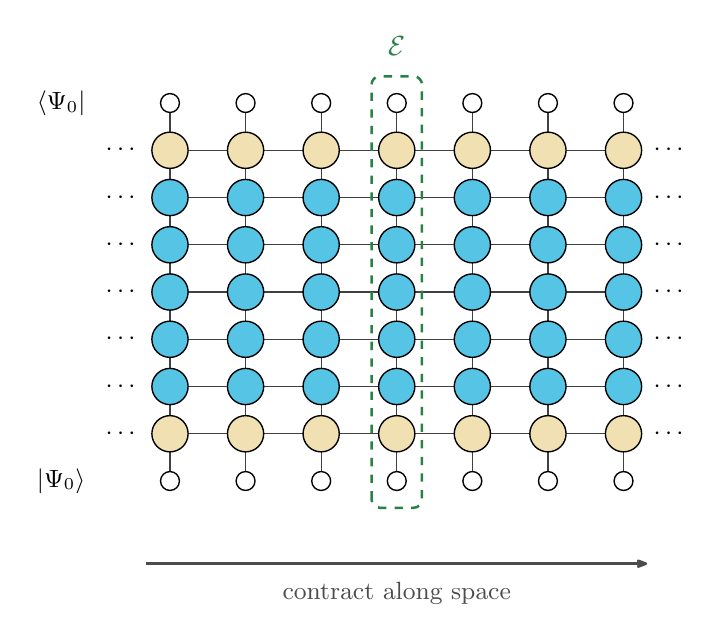
\begin{tikzpicture}[
    >={Stealth[round,length=2.0mm]},
    leg/.style={draw=black!75, line width=0.45pt},
    W/.style={circle, draw=black, fill=tnbulk, line width=0.5pt, minimum size=4.6mm, inner sep=0pt},
    B/.style={circle, draw=black, fill=tncool, line width=0.5pt, minimum size=4.6mm, inner sep=0pt},
    P/.style={circle, draw=black, fill=white, line width=0.5pt, minimum size=2.4mm, inner sep=0pt},
    vbox/.style={draw=tnbox, dashed, line width=0.9pt, rounded corners=3pt},
    tag/.style={font=\small},
  ]

  \foreach \i in {0,...,\NX} { \draw[leg] (\i*\DX,0) -- (\i*\DX,{8*\DY}); }
  \foreach \j in {1,...,7} { \draw[leg] (0,\j*\DY) -- (\NX*\DX,\j*\DY); }

  \foreach \i in {0,...,\NX} {
    \foreach \j in {1,7} { \node[B] at (\i*\DX,\j*\DY) {}; }
    \foreach \j in {2,...,6} { \node[W] at (\i*\DX,\j*\DY) {}; }
    \node[P] at (\i*\DX,0)       {};
    \node[P] at (\i*\DX,{8*\DY}) {};
  }

  \foreach \j in {1,...,7} {
    \node[tag] at (-0.60,\j*\DY)             {$\cdots$};
    \node[tag] at ({\NX*\DX+0.60},\j*\DY)    {$\cdots$};
  }

  % one spatial column = the transfer matrix
  \draw[vbox] ({3*\DX-0.32},-0.34) rectangle ({3*\DX+0.32},{8*\DY+0.34});
  \node[tag, tnbox, font=\normalsize] at ({3*\DX},{8*\DY+0.72}) {$\mathcal{E}$};

  \node[tag, anchor=east] at (-0.95,{8*\DY}) {$\bra{\Psi_0}$};
  \node[tag, anchor=east] at (-0.95,0)       {$\ket{\Psi_0}$};

  % contraction direction
  \draw[->, line width=1.0pt, black!70]
    (-0.3,-1.05) -- ({\NX*\DX+0.3},-1.05)
    node[midway, below=3pt, tag] {contract along space};

\end{tikzpicture}
\end{document}
